\setcounter{page}{1}
\artigofalse
\chapter{Introduction}
\label{chap:introduction}

\section{Background}

Soil science is experiencing a period of renaissance that started in the last 
decade \cite{HarteminkEtAl2008}. It is a result of a new global demand for soil 
information needed to solve what has been defined as the five major problems of
our time: food security, climate change, environmental degradation, water 
scarcity and threats to the biodiversity \cite{SanchezEtAl2009}. The Food and 
Agriculture Organization (\href{http://www.fao.org/index_en.htm}{FAO}) of the 
United Nations (\href{http://www.un.org/en/}{UN}), through the Global Soil 
Partnership (\href{http://www.fao.org/globalsoilpartnership/en/}{GSP}) project, 
is the main global demander of up-to-date soil information. The objective of 
FAO is to support and ensure the implementation of joint efforts that lead to 
the adoption of sustainable development goals for the soils \cite{FAO2012}. 
Digital soil mapping (DSM), \textit{the} \textit{creation and population of 
spatial soil information systems through the use of field and laboratory 
observational methods, coupled with spatial and non-spatial soil inference 
systems} \cite{LagacherieEtAl2007a}, a branch of pedometrics, a new emerging 
discipline of soil science that corresponds to the \textit{application of 
mathematical and statistical methods for the study of the distribution and 
genesis of soils} \cite{Heuvelink2003}, is the best alternative to meet this 
new demand for soil information. This is because DSM addresses the main 
problems of the classical approach of soil mapping \cite{Kempen2011}. First, 
DSM is data-centered (\textit{environmental-centered}) and gives emphasis on 
producing soil information according to the needs of soil information users 
(\textit{user-driven}). Second, DSM relies on using well documented statistical
models (\textit{reproducible research}) that allow treating the soil as a 
continuum (models of spatial variation). And third, DSM products can be made 
available at a lower cost in soil information systems with quantified 
uncertainty.

Several initiatives have been undertaken around the world in the last years to 
ensure the development and implementation of DSM. The main examples are the 
GlobalSoilMap.net consortium and ISRIC's Global Soil Information Facilities
(\href{http://www.isric.org/projects/global-soil-information-facilities-gsif}{GSIF}).
In Brazil, soil scientists created the Brazilian Network for Research in DSM 
(RedeMDS) with the main objective of generating synergy among Brazilian soil 
scientists to advance the research in DSM in Brazil \cite{RedeMDS2013}. Also, 
the two first job positions for assistant professors in Pedometrics and DSM in 
Brazilian universities were created in 2011 and 2013 \cite{UFRRJ2011,UFSM2012}. 
Unfortunately these local initiatives are not supported by any official 
government demand for up-to-date soil information in Brazil 
\cite{SamuelRosa2012}. Several economic, politic and cultural reasons have been 
pointed out to explain the lack of interest on soil information in Brazil since 
the 1980s \cite{Dalmolin1999, Ker1999, KerEtAl2003, Ramos2003, Espindola2008}, 
but their resolution is out of the scope of this thesis. Alike many other local
initiatives, the present thesis complies with the priorities defined by the 75 
soil scientists from 17 countries that came together in Rio de Janeiro on July 
2006 during the 2nd Global Workshop on Digital Soil Mapping, for whom developing
and implementing DSM depends on training students and experienced soil 
scientists, standardizing methods and measures, and building international 
collaboration \cite{Boettinger2004}.

\section{Digital soil mapping}

\subsection{Digital soil mapping framework}

In general terms, the DSM framework can be described as a series of seven steps 
as follows:

\begin{description}
  \item [{Step~0}] Identify a reality or problem entity: geographic region where
  pedometric techniques will be used to model the soil property(ies) distribution
  in the geographic and attribute spaces in a given time period;

  \item [{Step~1}] Develop a conceptual model of pedogenesis: verbal 
  representation of the reality or problem entity including the explicit 
  description of soil forming factors and processes that drive soil 
  characteristics and its spatial distribution pattern. This step relies on 
  gathering all environmental information available and applying concepts 
  (expert knowledge) of soil-landscape system, catenary soil development or 
  other theoretical model of explanation of soil spatial variation;

  \item [{Step~2}] Develop a mathematical representation: translate the verbal 
  representation of the reality or problem entity into a set of possible 
  mathematical representations. In this step we use the conceptual model of 
  pedogenesis to define the sample design and the number of soil observations 
  needed to calibrate the DSM model, collect predictor variables from available 
  environmental ancillary data (environmental covariates), specify model 
  structure (linear or non-linear) and define the techniques to be used in the 
  remainder of the DSM modelling activity (tests of independence, normality and 
  homoscedasticity, multicollinearity assessment, variable selection method, 
  goodness-of-fit measures, etc). Several of this tasks can be (and usually are)
  carried out with the aid of a data processing environment such as a computer;

  \item [{Step~3}] Develop a computer representation: translate the set of 
  mathematical representations of the reality or problem entity into a computer 
  representation, that is, a computer code or computer script. The computer 
  code is used to establish the communication between the DSM modeller (a human 
  being) and the data processing environment (a computer) where mathematical 
  representations and DSM model assessment tools are implemented. Developing a 
  computer code that describes all processing steps is at the core of the 
  concept of \textit{reproducible research} in DSM;

  \item [{Step~4}] Data analysis: run the computer code and evaluate the 
  outcomes. This includes the univariate analysis and selection of candidate 
  predictor variables, followed by its multivariate analysis, and evaluation of
  the adequacy of multivariate model(s), namely check model assumptions, look 
  for interactions between predictor variables, evaluate goodness-of-fit 
  measures and visually assess preliminary soil maps. Best performing DSM 
  model(s) are evaluated regarding their tenability (pedological evaluation) 
  and how well they represent the range of possible mathematical models. 
  Failure in this last assessment means that DSM model(s) have to be adjusted 
  and data analysis rerun, or can simply be discarded;

  \item [{Step~5}] Make predictions: application of best performing DSM model(s)
  to predict soil property values and confidence interval at unvisited locations;

  \item [{Step~6}] Statistical validation: validate the set of DSM models using
  existing independent field data and select the best performing model using a 
  statistical criterion. Best performing DSM model is assumed to be the best 
  mathematical representation of the reality or problem entity under 
  consideration. If previous steps have already allowed selecting a single best 
  performing DSM model, statistical validation is used only to assess model 
  accuracy;
  
  \item [{Step~7}] Reformulate the conceptual model of pedogenesis: selected 
  DSM model and prediction and uncertainty maps can provide new insights about 
  the reality or problem entity, and thus allow reformulating or improving the 
  verbal representation of the conceptual model of pedogenesis;
  
  \item [{Step~8}] Populate spatial soil information systems: point soil 
  observations, prediction and uncertainty maps, and metadata are used to 
  populate a spatial soil information system and made available for inspection 
  through different visualization techniques.
\end{description}

\subsection{Sources of uncertainty}

Despite the ease of building DSM models, their performance is quite variable and
usually lies between 20\% and 70\% of soil property variance explanation 
\cite{MooreEtAl1993, OdehEtAl1994, GesslerEtAl1995, McKenzieEtAl1999, 
GobinEtAl2001, SumflethEtAl2008, SunEtAl2012}. More complex non-linear models 
can be used to predict soil properties with greater accuracy, but they can be 
devoid of pedological information \cite{Grunwald2009}. Environmental covariates 
used to fit DSM models contain varying levels of error \cite{HeuvelinkEtAl1989}.
The diversity of statistical methods available for soil data analysis can lead 
to significantly different results \cite{ParkEtAl2002}. Soil observations can be
biased and poorly cover the geographic and feature spaces \cite{HenglEtAl2003a, 
BrusEtAl2007a}. Laboratory errors and positional accuracy of global positioning 
equipment can also affect prediction accuracy. Besides, some soil properties 
naturally contain more errors due to analytical procedures. In the case of 
particle-size distribution, the error is propagated to the fraction obtained by 
difference. Pre-treatments, such as organic matter oxidation, can change 
mineral structure \cite{MikuttaEtAl2005a}. The way compositional data is handled
also affects predicted values \cite{LarkEtAl2007}. Finally, the conceptual 
model of pedogenesis can be poorly formulated, and a poor DSM model can mislead 
its reformulation. Among all these sources of uncertainty, three of them are 
believed to have a major impact on model building and spatial prediction. They 
can be classified into three categories for didactic purposes: a) calibration 
observations, b) environmental covariates, and c) model structure.

\subsubsection*{Calibration observations}

Real-world soil data usually come from soil surveys where the number and 
location of calibration observations are defined based on the tacit knowledge 
of soil surveyors \cite{BrusEtAl2007a}. Several criteria are used by soil 
surveyors and, whenever possible, they attempt to obtain a nice distribution of 
observations in the geographic space. But this attempt is often held back by the
availability of financial resources, staff, time, presence of geographic 
accidents and prohibition of access in private properties \cite{KempenEtAl2012,
SamuelRosa2012}. Because of these issues, soil surveyors rarely use 
(geo)statistical criteria and usually obtain larger sampling densities in more 
complex and less known areas \cite{Rossiter2000}. This can cause both the 
selection of an insufficient as to an exaggerated number of samples 
\cite{vanGroenigenEtAl1999}. Sub-sampling leads to the construction of 
predictive models with little utility, giving a poor representation of the 
conceptual model of pedogenesis and low prediction accuracy, and over-sampling,
which allows building predictive models with great accuracy 
\cite{vanGroenigenEtAl1999}. But in both cases there is waste of financial 
resources, staff and time, what is highly undesirable because field sampling 
is the largest contributor to soil mapping costs \cite{vanGroenigenEtAl1999,
KempenEtAl2012, SamuelRosa2012}.

Several (geo)statistical criteria can be used to help defining appropriate 
calibration sample sizes and designs. For variographic analysis, it is 
recommended to use more than 100-250 (equidistant) observations, depending on 
the pattern of spatial distribution of the soil property under analysis 
\cite{WebsterEtAl2007}. Prior information on the spatial distribution of soil 
properties can be used coupled with optimization methods that minimize the 
kriging variance \cite{vanGroenigenEtAl1999, BrusEtAl2007a}. But it is also 
necessary to obtain a representative sample of the entire range of variation of 
the environmental covariates (attribute space) \cite{HenglEtAl2003a} to 
properly represent the conceptual model of pedogenesis. The variance of the 
estimated regression coefficients has also to be minimized \cite{BrusEtAl2007a}.
Finally, field work effort cannot overcome the available budget and the expected
gains of using soil maps \cite{KempenEtAl2012}. Due to these conflicting needs, 
model building in DSM is a multiple-objective optimization problem for which 
there is no unique solution, but a set of possible solutions (\textit{Pareto 
optimality}).

\subsubsection*{Covariates}

Several environmental covariates can be used to build DSM models, such as 
terrain attributes, geologic and land use maps, vegetation measures, surface 
reflectance, legacy soil data, among others \cite{McBratneyEtAl2003}. All of 
them contain errors. These errors derive from the methods of data generation, 
analytical procedures and inherent characteristics of each site. For example, 
digital elevation models (DEM) usually present larger errors in areas with steep
slopes, rough terrains and great elevations, and with dense forest cover or 
urbanized \cite{Florinsky1998, Toutin2000, FisherEtAl2006}. Interpolation of 
elevation data using kriging can produce spurious artefacts \cite{HenglEtAl2009}.
And stereoscopic correlation techniques produce DEMs with poorer quality than 
interferometric synthetic aperture radar \cite{HirtEtAl2010}.

Finding the ``optimal'' set of environmental covariates among several uncertain
environmental covariates can be accomplished using automated covariate selection
methods. The main issue is to select the most appropriate method. Some methods 
analyse all possible combinations of environmental covariates. Others simulate 
the process of natural selection (genetic algorithms) \cite{AndersenEtAl2010}. 
Cross-validation selects environmental covariates that produce the best 
predictions on test sets \cite{GuyonEtAl2003}. Other methods take into account 
the order in which the environmental covariates are added to (forward selection)
or removed from (backward elimination) the model \cite{LarkEtAl2007a}. And the 
stepwise method adds and removes environmental covariates until no further 
addition or removal results in significant change in the model 
\cite{VenablesEtAl2002}. But the number of problems associated with using these 
methods can be greater than the number of advantages \cite{Chatfield1995, 
LarkEtAl2007a}. In the multiple regression case the coefficients of 
determination and regression coefficients are overestimated, standard errors 
and \textit{P}-values are sub-estimated, and the multicollinearity problem is 
not solved \cite{Harrell2001a}. Besides, each method selects a different set of
environmental covariates, what constitutes a source of uncertainty regarding 
model specification \cite{Harrell2001a}.

\section{Content of the thesis}

\subsection{Objectives and research questions}

Translating verbal representations of conceptual models that describe reality 
into mathematical representations of these models is a key step in DSM. There 
are several sources of uncertainty that may affect the development of such 
mathematical representations. These sources of uncertainty can be classified 
into three categories for didactic purposes: a) calibration observations, b) 
environmental covariates and c) model structure. The general objective of this 
project is to evaluate these three main sources of uncertainty in DSM under 
different database scenarios. This general objective can be divided into three 
specific objectives with their respective research questions:

\begin{enumerate}
  \item Identify appropriate calibration sample sizes and designs;

  \subitem [{Research\ Question}] How calibration sample size and sampling 
  design affect model composition, prediction accuracy and monetary cost?

  \item Determine the accuracy of freely available covariates and their 
  suitability for DSM;

  \subitem [{Research\ Question}] How much accuracy improvement is achieved 
  when more detailed covariates are used?

  \item Identify appropriate covariate selection methods to build linear 
  predictive models;

  \subitem [{Research\ Question}] How covariate selection methods affect model 
  composition and prediction accuracy?
\end{enumerate}

\subsection{Study area and database}

The soil database used comes from a study area in the southern edge of the 
plateau of the Paraná Sedimentary Basin, in the state of Rio Grande do Sul, 
Brazil. This study area is a small catchment (1,892 ha) which constitutes 60\% 
of the entire catchment of one of the water reservoirs of the city of Santa 
Maria (\ref{fig:location-intro}). Climate is classified as Cfa (Köppen climate 
classification - subtropical humid without a dry season) with mean annual 
temperature of $19.3^{\circ}$C, and mean annual precipitation of 1,708 mm well 
distributed throughout the year \cite{Maluf2000}. Relief varies between plain 
(slope between 0 and 3\%) and mountainous (slope between 45 and 100\%), and 
elevations range between 139 and 475 m. There are three main geological 
formations which consist of (a) basic, intermediate and acid igneous rocks 
(rhyolite-rhyodacite and andesite-basalt) of the Cretaceous period; (b) 
consolidated sedimentary rocks (aeolian and fluvial sandstones) of the Triassic
and Jurassic periods; and (c) non-consolidated (fluvial and colluvial deposits)
of the Quaternary period \cite{GasparettoEtAl1988, MacielFilho1990, Sartori2009}.
Forest areas occupy more than half of the study area, followed by native 
grassland, shrubland, farmland, forestry, urban areas and artificial water 
bodies \cite{SamuelRosaEtAl2011a}.

\begin{figure}[!ht]
    \centering
    \begin{minipage}[b]{95mm}
      \subcaption{}
      \label{fig:brazil}
      \centering
      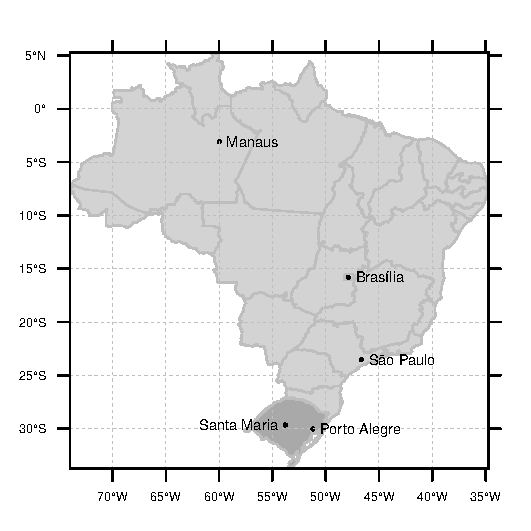
\includegraphics[width=90mm]{chap01FIG1a}
    \end{minipage}
    \begin{minipage}[b]{95mm}
      \subcaption{}
      \label{fig:points}
      \centering
      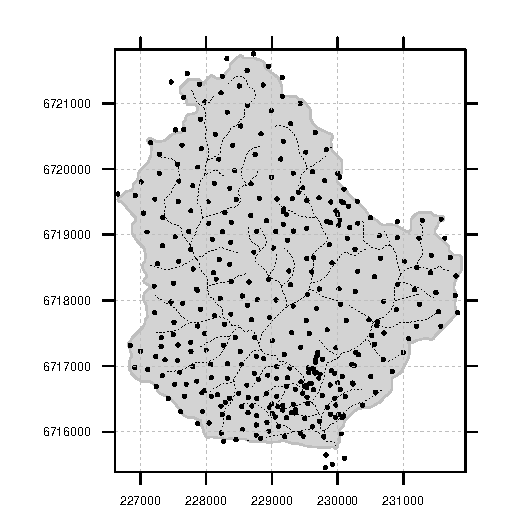
\includegraphics[width=90mm]{chap01FIG1b}
    \end{minipage}
  \caption{Location of the study area (a) in the central region of the 
  southernmost Brazilian state, Rio Grande do Sul, and the spatial distribution 
  of the $n=350$ point soil observations (b) made between the years of 2008 and
  2011 as part of soil and land use mapping projects.}
  \label{fig:location-intro}
\end{figure}

The soil database is composed by $n=350$ point observations. They were sampled 
during a soil and land use survey started in 2008 and published in the scale of
1:30,000 \cite{SamuelRosaEtAl2011a, MiguelEtAl2012}. Soil data includes 
particle size distribution, organic carbon content, bulk density, and effective 
cation exchange capacity. Environmental covariates include 20 data layers freely
available for the study area. They include information on relief, vegetation, 
land use, geology, soil parent material, soil (taxa) and intimately-associated 
surface conditions.

\subsection{Outline}

The thesis is composed of three chapters. Each chapter deals with one specific 
research question and specific objective. Chapter 1 will deal with assessing 
whether investing in more accurate covariates improves prediction accuracy. 
Chapter 2 will deal with identifying appropriate calibration sample sizes and 
sampling designs for building DSM models for mapping soil properties. Chapter 3 
will deal with evaluating automated methods used to select covariates to build 
linear DSM models on how they affect model composition and prediction accuracy.